\PassOptionsToPackage{unicode=true}{hyperref} % options for packages loaded elsewhere
\PassOptionsToPackage{hyphens}{url}
%
\documentclass[]{article}
\usepackage[a4paper, total={6in, 8in}]{geometry}
\usepackage[UTF8]{ctex}
\usepackage{lmodern}
\usepackage{amssymb,amsmath}
\usepackage{ifxetex,ifluatex}
\usepackage{fixltx2e} % provides \textsubscript
\ifnum 0\ifxetex 1\fi\ifluatex 1\fi=0 % if pdftex
  \usepackage[T1]{fontenc}
  \usepackage[utf8]{inputenc}
  \usepackage{textcomp} % provides euro and other symbols
\else % if luatex or xelatex
  \usepackage{unicode-math}
  \defaultfontfeatures{Ligatures=TeX,Scale=MatchLowercase}
\fi
% use upquote if available, for straight quotes in verbatim environments
\IfFileExists{upquote.sty}{\usepackage{upquote}}{}
% use microtype if available
\IfFileExists{microtype.sty}{%
\usepackage[]{microtype}
\UseMicrotypeSet[protrusion]{basicmath} % disable protrusion for tt fonts
}{}
\IfFileExists{parskip.sty}{%
\usepackage{parskip}
}{% else
\setlength{\parindent}{0pt}
\setlength{\parskip}{6pt plus 2pt minus 1pt}
}
\usepackage{hyperref}
\hypersetup{
            pdfborder={0 0 0},
            breaklinks=true}
\urlstyle{same}  % don't use monospace font for urls
\usepackage{color}
\usepackage{fancyvrb}
\newcommand{\VerbBar}{|}
\newcommand{\VERB}{\Verb[commandchars=\\\{\}]}
\DefineVerbatimEnvironment{Highlighting}{Verbatim}{commandchars=\\\{\}}
% Add ',fontsize=\small' for more characters per line
\newenvironment{Shaded}{}{}
\newcommand{\AlertTok}[1]{\textcolor[rgb]{1.00,0.00,0.00}{\textbf{#1}}}
\newcommand{\AnnotationTok}[1]{\textcolor[rgb]{0.38,0.63,0.69}{\textbf{\textit{#1}}}}
\newcommand{\AttributeTok}[1]{\textcolor[rgb]{0.49,0.56,0.16}{#1}}
\newcommand{\BaseNTok}[1]{\textcolor[rgb]{0.25,0.63,0.44}{#1}}
\newcommand{\BuiltInTok}[1]{#1}
\newcommand{\CharTok}[1]{\textcolor[rgb]{0.25,0.44,0.63}{#1}}
\newcommand{\CommentTok}[1]{\textcolor[rgb]{0.38,0.63,0.69}{\textit{#1}}}
\newcommand{\CommentVarTok}[1]{\textcolor[rgb]{0.38,0.63,0.69}{\textbf{\textit{#1}}}}
\newcommand{\ConstantTok}[1]{\textcolor[rgb]{0.53,0.00,0.00}{#1}}
\newcommand{\ControlFlowTok}[1]{\textcolor[rgb]{0.00,0.44,0.13}{\textbf{#1}}}
\newcommand{\DataTypeTok}[1]{\textcolor[rgb]{0.56,0.13,0.00}{#1}}
\newcommand{\DecValTok}[1]{\textcolor[rgb]{0.25,0.63,0.44}{#1}}
\newcommand{\DocumentationTok}[1]{\textcolor[rgb]{0.73,0.13,0.13}{\textit{#1}}}
\newcommand{\ErrorTok}[1]{\textcolor[rgb]{1.00,0.00,0.00}{\textbf{#1}}}
\newcommand{\ExtensionTok}[1]{#1}
\newcommand{\FloatTok}[1]{\textcolor[rgb]{0.25,0.63,0.44}{#1}}
\newcommand{\FunctionTok}[1]{\textcolor[rgb]{0.02,0.16,0.49}{#1}}
\newcommand{\ImportTok}[1]{#1}
\newcommand{\InformationTok}[1]{\textcolor[rgb]{0.38,0.63,0.69}{\textbf{\textit{#1}}}}
\newcommand{\KeywordTok}[1]{\textcolor[rgb]{0.00,0.44,0.13}{\textbf{#1}}}
\newcommand{\NormalTok}[1]{#1}
\newcommand{\OperatorTok}[1]{\textcolor[rgb]{0.40,0.40,0.40}{#1}}
\newcommand{\OtherTok}[1]{\textcolor[rgb]{0.00,0.44,0.13}{#1}}
\newcommand{\PreprocessorTok}[1]{\textcolor[rgb]{0.74,0.48,0.00}{#1}}
\newcommand{\RegionMarkerTok}[1]{#1}
\newcommand{\SpecialCharTok}[1]{\textcolor[rgb]{0.25,0.44,0.63}{#1}}
\newcommand{\SpecialStringTok}[1]{\textcolor[rgb]{0.73,0.40,0.53}{#1}}
\newcommand{\StringTok}[1]{\textcolor[rgb]{0.25,0.44,0.63}{#1}}
\newcommand{\VariableTok}[1]{\textcolor[rgb]{0.10,0.09,0.49}{#1}}
\newcommand{\VerbatimStringTok}[1]{\textcolor[rgb]{0.25,0.44,0.63}{#1}}
\newcommand{\WarningTok}[1]{\textcolor[rgb]{0.38,0.63,0.69}{\textbf{\textit{#1}}}}
\usepackage{graphicx,grffile}
\makeatletter
\def\maxwidth{\ifdim\Gin@nat@width>\linewidth\linewidth\else\Gin@nat@width\fi}
\def\maxheight{\ifdim\Gin@nat@height>\textheight\textheight\else\Gin@nat@height\fi}
\makeatother
% Scale images if necessary, so that they will not overflow the page
% margins by default, and it is still possible to overwrite the defaults
% using explicit options in \includegraphics[width, height, ...]{}
\setkeys{Gin}{width=\maxwidth,height=\maxheight,keepaspectratio}
\setlength{\emergencystretch}{3em}  % prevent overfull lines
\providecommand{\tightlist}{%
  \setlength{\itemsep}{0pt}\setlength{\parskip}{0pt}}
\setcounter{secnumdepth}{0}
% Redefines (sub)paragraphs to behave more like sections
\ifx\paragraph\undefined\else
\let\oldparagraph\paragraph
\renewcommand{\paragraph}[1]{\oldparagraph{#1}\mbox{}}
\fi
\ifx\subparagraph\undefined\else
\let\oldsubparagraph\subparagraph
\renewcommand{\subparagraph}[1]{\oldsubparagraph{#1}\mbox{}}
\fi

% set default figure placement to htbp
\makeatletter
\def\fps@figure{htbp}
\makeatother


\title{数据结构与算法I 实验8}
\author{2019201409 于倬浩}

\begin{document}
\maketitle


\tableofcontents

\hypertarget{header-n4}{%
\subsection{一、实验内容}\label{header-n4}}

实现二项堆的各项操作。

额外实现了可视化,结果动图位于\texttt{./Result.gif}。

\hypertarget{header-n13}{%
\subsection{二、实现操作\&接口}\label{header-n13}}

核心节点类定义如下:

\begin{Shaded}
\begin{Highlighting}[]
\KeywordTok{struct}\NormalTok{ node\{}
    \DataTypeTok{int}\NormalTok{ deg;}
    \CommentTok{//当前节点的度数}
\NormalTok{    node *fa, *ch, *sib;}
    \CommentTok{//分别表示当前节点的父亲、最左儿子、兄弟节点}
    \DataTypeTok{int}\NormalTok{* val;}
    \CommentTok{//指向当前节点的数据域的指针}
\NormalTok{\};}
\KeywordTok{typedef}\NormalTok{ node* BinomialHeap; }\CommentTok{//简略定义}
\end{Highlighting}
\end{Shaded}

注意到数据类型\texttt{BinomialHeap}在不维护其他卫星数据的情况下,只有一个\texttt{node*}是有效的数据。因此,在仅需最基本的操作的情况下,无需另外定义\texttt{BinomialHeap}类,可以使代码减少不必要的细节,更为简洁。

各种接口:

\begin{Shaded}
\begin{Highlighting}[]
\KeywordTok{inline} \DataTypeTok{void}\NormalTok{ init();}
\CommentTok{// 定义二项堆前必须调用init()初始化哨兵节点}

\KeywordTok{inline}\NormalTok{ BinomialHeap binomialHeapUnion(BinomialHeap a, BinomialHeap b);}
\CommentTok{// 合并a、b两个堆(不进行任何拷贝操作)并返回新堆}

\KeywordTok{inline} \DataTypeTok{void}\NormalTok{ binomialHeapInsert(BinomialHeap& h, }\DataTypeTok{int}\NormalTok{ val);}
\CommentTok{// 向堆h中插入值val}
\CommentTok{// *由于可能修改当前堆的结构,传入引用}

\KeywordTok{inline} \DataTypeTok{void}\NormalTok{ decreaseKey(BinomialHeap h, node* key, }\DataTypeTok{int}\NormalTok{ val);}
\CommentTok{// 将堆h中的key节点键值改为val}
\CommentTok{// 使用assert保证val必须不大于原值,否则程序退出}

\KeywordTok{inline} \DataTypeTok{int}\NormalTok{ extractMin(BinomialHeap &h);}
\CommentTok{// 弹出最小值}
\CommentTok{// *由于可能修改当前堆的结构,传入引用}

\KeywordTok{inline} \DataTypeTok{void}\NormalTok{ binomialHeapErase(BinomialHeap& h, node *key);}
\CommentTok{// 从h中删除key节点}
\CommentTok{// *由于可能修改当前堆的结构,传入引用}
\end{Highlighting}
\end{Shaded}

为了代码简洁起见,并没有采取封装设计,堆合并更为简洁。

\hypertarget{header-n17}{%
\subsection{三、算法设计}\label{header-n17}}

大致思路采取第三版CLRS上二项堆章节的讲解。

首先有一个重要的操作\texttt{binomialLink(a,b)}表示把b设为a的父亲,且此时a一定是b度数最大的儿子(每次只会将度数相邻的节点进行\texttt{binomialLink}),在代码里实现为\texttt{node}类的成员函数:

\begin{Shaded}
\begin{Highlighting}[]
\KeywordTok{inline}\NormalTok{ node* binomialLink(node *x) \{}
    \ControlFlowTok{if}\NormalTok{(x == null) }\ControlFlowTok{return}\NormalTok{ null;}
\NormalTok{    x->fa = }\KeywordTok{this}\NormalTok{;}
\NormalTok{    x->sib = ch;}
\NormalTok{    ch = x;}
\NormalTok{    ++deg;}
    \ControlFlowTok{return} \KeywordTok{this}\NormalTok{;}
\NormalTok{\}}
\end{Highlighting}
\end{Shaded}

\begin{itemize}
\item
  合并操作\texttt{binomialHeapUnion}

  \begin{itemize}
  \item
    \texttt{mergeHeap(a,\ b)}:将两个二项堆a、b的二项树构成的森林进行简单的合并,确保合并后的链上度数递增。

    此时对于任意度数,最多有两棵树具有相同的度数。

    由于二项树的节点度数维持在\(O(lgn)\)级别,该操作时间复杂度为\(O(lgn)\)。
  \item
    \texttt{binomialHeapUnion(a,\ b)}:用户需要调用的合并堆操作。

    首先利用\texttt{mergeHeap}拉出一条链,考虑链上的二项树度数递增,如果相邻的两棵树度数已经不同,那么不需要处理。如果相邻的两棵树度数相同,则利用之前的\texttt{binomialLink},将键值较小的节点设为父亲即可,既维护了堆性质,又维护了二项堆不能有度数相同的二项树性质。具体实现上,只需维护当前节点的前一个、后一个节点(\texttt{prev\_x}、\texttt{next\_x}),然后比较度数,分类讨论即可。时间复杂度\( O(lgn)\)。
  \end{itemize}
\end{itemize}

\begin{itemize}
\item
  插入操作\texttt{binomialHeapInsert}

  使用合并操作构造即可。

\begin{Shaded}
\begin{Highlighting}[]
\KeywordTok{inline} \DataTypeTok{void}\NormalTok{ binomialHeapInsert(BinomialHeap& h, }\DataTypeTok{int}\NormalTok{ val) \{}
\NormalTok{    BinomialHeap n = }\KeywordTok{new}\NormalTok{ node; }\CommentTok{// 新建节点}
\NormalTok{    n->val = }\KeywordTok{new} \DataTypeTok{int}\NormalTok{(val); }\CommentTok{// 新建数据域}
\NormalTok{    h = binomialHeapUnion(h, n);}
\NormalTok{\}}
\end{Highlighting}
\end{Shaded}
\item
  减小键值\texttt{decreaseKey}

  实际上就是从某个节点开始,不断跳父亲指针,如果当前节点的键值小于父亲的,那么交换指向数据的指针(之所以不交换节点本身的指针,是由于每个节点都有父亲指针,如果修改了树的结构,那么复杂度退化为\(O(lg^2n)\);不交换数据是因为在维护的数据较大时,交换指针可以保证运行效率)。
\item
  提取最小值\texttt{extractMin}

  首先需要遍历所有二项树的根,找到最小的一个。接下来删掉这颗树的根,将树根的儿子拉成一条链,将其他所有二项树根拉成另一条链,再使用\texttt{binomialHeapUnion}操作,将两条链构成的二项树森林合并度数相同的节点,即维持了二项堆的性质。
\item
  删除节点\texttt{binomialHeapErase}

  只需利用\texttt{decreaseKey}和\texttt{extractMin}构造全局最小值然后弹出即可。

\begin{Shaded}
\begin{Highlighting}[]
\KeywordTok{inline} \DataTypeTok{void}\NormalTok{ binomialHeapErase(BinomialHeap& h, node *key) \{}
\NormalTok{    decreaseKey(h, key, }\DecValTok{-2147483648}\NormalTok{);}
\NormalTok{    extractMin(h);}
\NormalTok{\}}
\end{Highlighting}
\end{Shaded}
\end{itemize}

\hypertarget{header-n21}{%
\subsection{四、测试\&可视化}\label{header-n21}}

对于需要使用节点指针作为参数的几项操作,由于不便可视化,使用gdb输出节点地址,然后直接输入指针地址进行测试。

对于基本的堆插入/弹出操作,使用\texttt{GraphViz}处理,每次操作后实时展示二项树森林的结构,可以确保堆合并/插入/弹出等操作的正确性。而其他几项操作又主要依赖合并操作,因此,在确定了合并/弹出最小值两个操作的正确性后,其他操作的正确性也就有了保障。

可视化的具体步骤是,首先造了一组简单的操作序列,含有若干插入/弹出操作。每次操作后,调用\texttt{dotify()}生成\texttt{.dot}文件,接下来使用\texttt{GraphViz}的实时预览插件,即可做到每次操作后生成结果,例如下图:

\begin{figure}
\centering
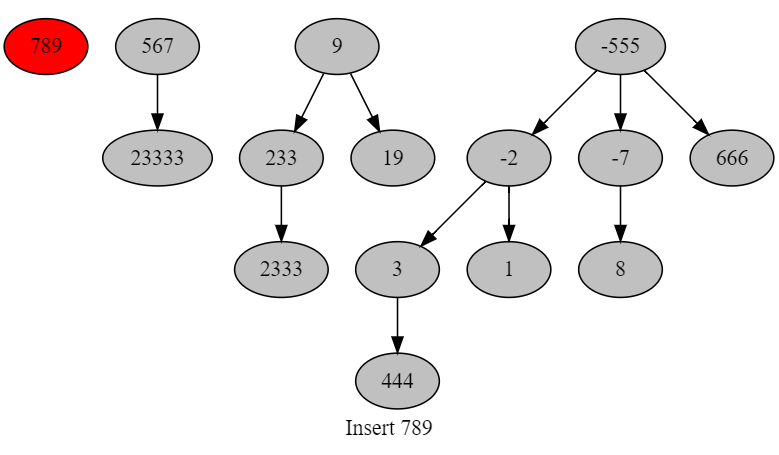
\includegraphics{C:/Users/zhuoh/Desktop/Docs/ds-lab8/Lab8_2019201409_于倬浩.assets/image-20201209233850483.png}
\caption{可视化结果示例}
\end{figure}

对于另一组数据,包含了一些插入和弹出操作,制作成动图,为文件夹内的\texttt{Result.gif}。

\end{document}
